\documentclass[8pt, handout]{beamer} 


%% Math packages
%%
\usepackage{amsmath,amsthm,amssymb}
% Removes the "Too many math alphabets used in version normal" error.
\newcommand\hmmax{0}
\newcommand\bmmax{0}
\usepackage[new]{old-arrows}
\usepackage{cancel}
\usepackage{mathdots}
\usepackage{venndiagram}
\usepackage{mathrsfs}          % Math script font

% Graphics
%%
\graphicspath{{./}{figs/}}
\usepackage{graphicx}
\usepackage{tikz}
\usetikzlibrary{arrows}
\usetikzlibrary{decorations.markings}
\usetikzlibrary{decorations.pathreplacing}
\usetikzlibrary{patterns}
\usetikzlibrary{shapes.geometric}
\usetikzlibrary{matrix}
\usepackage{tikz-3dplot}
\usepackage{tkz-graph}
\usepackage{tikz-cd}

%% Colors (most are in colors.tex file)
%%
\usepackage{xcolor}
\usepackage{color}
\usepackage{visualalgebra}  %% Put this *after* the TikZ packages
\usepackage{visualalgebraslides}  %% Put this *after* "visualalgebra"

%% Page layout packages
%%
\usepackage{url}
\usepackage{multicol}
\usepackage{multirow}
\usepackage[numbers,square,sort&compress]{natbib}

%% Font and formatting packages
%%
\usepackage[english]{babel}    % Removing this causes compiler error
\usepackage{alltt}             % Like verbatim, but excludes \ and { }
\usepackage{enumerate}         % [shortlabels] option??
\usepackage{comment}
\usepackage{soul}              % strikeout text
\usepackage{bm}                % Bold math
\usepackage[T1]{fontenc}
\usepackage{relsize}

%% Fixes the \mathbf{} not working for fonts under 10pt
\usepackage{cmbright}
\fontencoding{OT1}\fontfamily{cmbr}\selectfont %to load ot1cmbr.fd
\DeclareFontShape{OT1}{cmbr}{bx}{n}{% change bx definition
<->cmbrbx10%
}{}
\normalfont

\makeatletter
\renewcommand*\env@matrix[1][\arraystretch]{%
  \edef\arraystretch{#1}%
  \hskip -\arraycolsep
  \let\@ifnextchar\new@ifnextchar
  \array{*\c@MaxMatrixCols c}}
\makeatother


%%=======================================================================

%% Beamer packages
%%
\mode<presentation>
{
  \usetheme{boadilla} 
  \useinnertheme{rectangles}
  \usecolortheme{dolphin}
}

\setbeamersize{text margin left=6mm}
\setbeamersize{text margin right=6mm}
\setbeamersize{sidebar width right=0mm}
\setbeamersize{sidebar width left=0mm}
\setbeamertemplate{navigation symbols}{}

\def\newblock{\hskip .11em plus .33em minus .07em}

% Other options: ball, circle, square 
\setbeamertemplate{enumerate items}[default]
%\setbeamercolor{enumerate subitem}{fg=red!80!black}
\def\opacity{0.5}
%setbeamercovered{transparent}
\setbeamercovered{invisible}

\newcommand{\Pause}{\pause}      %% Comment this out => lots more page breaks
% \newcommand{\Pause}{}

\AtBeginSection[]{
  \begin{frame}
  \vfill
  \centering
  \begin{beamercolorbox}[sep=8pt,center,shadow=true,rounded=true]{title}
    \usebeamerfont{title}\insertsectionhead\par%
  \end{beamercolorbox}
  \vfill
  \end{frame}
}


%%====================================================================

\title[Homomorphisms!]{Isomorphisms!}
\subtitle{(but first, homomorphisms!)}

\author[\href{mailto:sbagley@westminsteru.edu}{S. Bagley}]
       {\href{mailto:sbagley@westminsteru.edu}{Spencer Bagley}}

\institute[Westminster] { 
  \normalsize With many thanks to Matthew Macauley, \\
  \url{http://www.math.clemson.edu/~macaule/}}

\date[10 Mar 2025]{10 Mar 2025}

\begin{document}

\frame{\titlepage}

%%====================================================================

\begin{frame}{Goals for today:}
  \begin{enumerate}
    \item We have sure said the word ``isomorphic'' a lot
    \item Let's figure out what that \Alert{actually} means
    \item Lots of examples
    \item Some problems to play with
  \end{enumerate}
\end{frame}

%%====================================================================
\section{First, something from the hw}
%%====================================================================

\begin{frame}{The quotient $G/Z(G)$ can \emph{never} be a nontrivial cyclic subgroup}
  
  \begin{block}{From homework:}
    If $G/Z(G)$ is cyclic, then $G$ is abelian.
  \end{block}

  \vspace{-4mm}

  %% Shoebox diagram of G/Z(G), and the subgroup lattice of C7xC6.
  \[
  \begin{tikzpicture}[scale=.7]
    %%
    \newcommand\Hh{6.5} % height of 42
    \newcommand\Hg{5.5} % height of 21
    \newcommand\Hf{4.5} % height of 14
    \newcommand\He{3.5} % height of 7
    \newcommand\Hd{2.5} % height of 6
    \newcommand\Hc{1.5} % height of 3
    \newcommand\Hb{1} % height of 2
    \newcommand\Ha{0} % height of 1
    \tikzstyle{every node}=[font=\footnotesize,anchor=south]
    \begin{scope}[shift={(0,0)},scale=1.5,xscale=1.1]
      \node at (2.25,3.25)
            {\normalsize \emph{$\bm{G/Z(G)=\<gZ\>}$, where $Z\!=\!Z(G)$}};
      \draw[thin] (0,0) rectangle (4.5,3);
      \draw[thin,fill=faded] (0,0) rectangle (4.5,.5);
      \draw[thin] (0,2.5) to (4.5,2.5);
      \draw[thin] (0,1.5) to (4.5,1.5);
      \draw[thin] (0,1) to (4.5,1);
      %%
      \node[anchor=west] at (.2,2.77) {$\bullet\;g^{n-1}$};
      \node[anchor=west] at (.85,2.77) {$\bullet\;g^{n-1}\!z_1$};
      \node[anchor=west] at (1.7,2.77) {$\bullet\;g^{n-1}\!z_2$};
      \node[anchor=west] at (2.55,2.77) {$\bullet\;g^{n-1}\!z_3$};
      \node[anchor=west] at (3.35,2.77) {$\cdots$};
      \node[anchor=east] at (4.43,2.77) {\normalsize $\bm{g^{n-1}\!Z}$};
      %%
      \node at (2.25,1.77) {\Large $\bm\vdots$};
      %%
      \node[anchor=west] at (.2,1.27) {$\bullet\;g^2$};
      \node[anchor=west] at (.85,1.27) {$\bullet\;g^2z_1$};
      \node[anchor=west] at (1.7,1.27) {$\bullet\;g^2\!z_2$};
      \node[anchor=west] at (2.55,1.27) {$\bullet\;g^2\!z_3$};
      \node[anchor=west] at (3.35,1.27) {$\cdots$};
      \node[anchor=east] at (4.43,1.27) {\normalsize $\bm{g^2\!Z}$};
      %%
      \node[anchor=west] at (.2,.77) {$\bullet\;g$};
      \node[anchor=west] at (.85,.77) {$\bullet\;gz_1$};
      \node[anchor=west] at (1.7,.77) {$\bullet\;gz_2$};
      \node[anchor=west] at (2.55,.77) {$\bullet\;gz_3$};
      \node[anchor=west] at (3.35,.77) {$\cdots$};
      \node[anchor=east] at (4.43,.77) {\normalsize $\bm{gZ}$};
      %%
      \node[anchor=west] at (.2,.27) {$\bullet\;e$};
      \node[anchor=west] at (.85,.27) {$\bullet\;z_1$};
      \node[anchor=west] at (1.7,.27) {$\bullet\;z_2$};
      \node[anchor=west] at (2.55,.27) {$\bullet\;z_3$};
      \node[anchor=west] at (3.35,.27) {$\cdots$};
      \node[anchor=east] at (4.43,.27) {\normalsize $\bm{Z}$};
      %%
    \end{scope}
    %%
    \begin{scope}[shift={(11.8,-1.25)},scale=1,shorten >= -1pt, shorten <= -1pt,xscale=.7,yscale=1.15]
      \tikzstyle{every node}=[font=\footnotesize]
      \node(G) at (-1.75,\Hh) {\small $C_7\!\rtimes\!C_6$};
      \node(C7-C3) at (-4.25,\Hg) {\small $C_7\!\rtimes\!C_3$};
      \node(D7) at (-1.75,\Hf) {\small $D_7$};
      \node(C7) at (-4.25,\He) {\small $C_7$};
      \node(C3-1) at (-1.25,\Hc) {$C_3$};
      \node(C3-2) at (-.75,\Hc) {$C_3$};
      \node(C3-3) at (-.25,\Hc) {$C_3$};
      \node(C3-4) at (.25,\Hc) {$C_3$};
      \node(C3-5) at (.75,\Hc) {$C_3$};
      \node(C3-6) at (1.25,\Hc) {$C_3$};
      \node(C3-7) at (1.75,\Hc) {$C_3$};
      \node(C6-1) at (3.25,\Hd) {$C_6$};
      \node(C6-2) at (3.75,\Hd) {$C_6$};
      \node(C6-3) at (4.25,\Hd) {$C_6$};
      \node(C6-4) at (4.75,\Hd) {$C_6$};
      \node(C6-5) at (5.25,\Hd) {$C_6$};
      \node(C6-6) at (5.75,\Hd) {$C_6$};
      \node(C6-7) at (6.25,\Hd) {$C_6$};
      \node(C2-1) at (3.25,\Hb) {$C_2$};
      \node(C2-2) at (3.75,\Hb) {$C_2$};
      \node(C2-3) at (4.25,\Hb) {$C_2$};
      \node(C2-4) at (4.75,\Hb) {$C_2$};
      \node(C2-5) at (5.25,\Hb) {$C_2$};
      \node(C2-6) at (5.75,\Hb) {$C_2$};
      \node(C2-7) at (6.25,\Hb) {$C_2$};
      \node(1) at (0,\Ha) {\small $C_1$};
      \draw[faded] (G) to (C7-C3);
      \draw[faded] (G) to (D7);
      \draw[faded] (G) to (C6-1);
      \draw[faded] (G) to (C6-2);
      \draw[faded] (G) to (C6-3);
      \draw[faded] (G) to (C6-4);
      \draw[faded] (G) to (C6-5);
      \draw[faded] (G) to (C6-6);
      \draw[faded] (G) to (C6-7);
      \draw[faded] (D7) to (C7);
      \draw[faded] (D7) to (C2-1);
      \draw[faded] (D7) to (C2-2);
      \draw[faded] (D7) to (C2-3);
      \draw[faded] (D7) to (C2-4);
      \draw[faded] (D7) to (C2-5);
      \draw[faded] (D7) to (C2-6);
      \draw[faded] (D7) to (C2-7);
      \draw[faded] (C7-C3) to (C7);
      \draw[faded] (C7) to (1);
      \draw[faded] (C7-C3) to (C3-1);
      \draw[faded] (C7-C3) to (C3-2);
      \draw[faded] (C7-C3) to (C3-3);
      \draw[faded] (C7-C3) to (C3-4);
      \draw[faded] (C7-C3) to (C3-5);
      \draw[faded] (C7-C3) to (C3-6);
      \draw[faded] (C7-C3) to (C3-7);
      \draw[faded] (C6-1) to (C2-1);
      \draw[faded] (C6-2) to (C2-2);
      \draw[faded] (C6-3) to (C2-3);
      \draw[faded] (C6-4) to (C2-4);
      \draw[faded] (C6-5) to (C2-5);
      \draw[faded] (C6-6) to (C2-6);
      \draw[faded] (C6-7) to (C2-7);
      \draw[faded] (C6-1) to (C3-1);
      \draw[faded] (C6-2) to (C3-2);
      \draw[faded] (C6-3) to (C3-3);
      \draw[faded] (C6-4) to (C3-4);
      \draw[faded] (C6-5) to (C3-5);
      \draw[faded] (C6-6) to (C3-6);
      \draw[faded] (C6-7) to (C3-7);
      \draw[faded] (1) to (C3-1);
      \draw[faded] (1) to (C3-2);
      \draw[faded] (1) to (C3-3);
      \draw[faded] (1) to (C3-4);
      \draw[faded] (1) to (C3-5);
      \draw[faded] (1) to (C3-6);
      \draw[faded] (1) to (C3-7);
      \draw[faded] (1) to (C2-1);
      \draw[faded] (1) to (C2-2);
      \draw[faded] (1) to (C2-3);
      \draw[faded] (1) to (C2-4);
      \draw[faded] (1) to (C2-5);
      \draw[faded] (1) to (C2-6);
      \draw[faded] (1) to (C2-7);
    \end{scope}
    \end{tikzpicture}
%    \caption{Left: If $G/Z(G)$ is cyclic, then arbitrary elements $a,b\in G$ must have the form $a=g^iz_1$ and $b=g^jz_2$ for some $i,j\in\Z$ and $z_1,z_2\in Z(G)$. Right: The center of $G=C_7\!\rtimes\!C_6$ cannot be $C_7\!\rtimes\!C_3$, $D_7$, and $C_7$ because these all have cyclic quotients with $G$.}\label{fig11:F-contraction-lemma}
  \]
  Note that if $G$ is abelian, then $Z(G)=G$.
  
\end{frame}


%%====================================================================
\section{Definition and notation time!}
%%====================================================================

\begin{frame}{Functions!}

  Nothing on this slide is specific to abstract algebra. \pause
  
  \begin{block}{Extremely technical definition}
    Let $A, B$ be two \Alert{sets}. \pause A \Alert{function} $f$ is a subset of the Cartesian product $A \times B$ such that: \pause
    \begin{itemize}
      \item for all $a\in A$, there exists $b\in B$ such that $(a, b) \in f$
      \pause \hfill \emph{\Balert{(existence of images)}} \pause
      \item if $(a, b) \in f$ and $(a, b') \in f$, then $b = b'$ \hfill \emph{\Balert{(uniqueness of images)}}
    \end{itemize}
  \end{block} \pause

  This definition sucks and I hate it. \pause

  \begin{block}{Less technical but more useful definition}
    Let $A, B$ be two sets. A function $f$ is a \Alert{map} from $A$ to $B$ such that: \pause
    \begin{itemize}
      \item for all $a\in A$, there exists $b\in B$ such that $f(a) = b$
      \pause \hfill \emph{\Balert{(existence of images)}} \pause
      \item if $f(a) = b$ and $f(a) = b'$, then $b = b'$ \hfill \emph{\Balert{(uniqueness of images)}}
    \end{itemize}
  \end{block} \pause

  (Just don't ask me to formally explain what a ``map'' is.) \pause

  \begin{exampleblock}{Moral definition}
    \begin{itemize}
      \item $f$ sends elements of $A$ (inputs) to elements of $B$ (outputs)
      \pause \hfill \emph{\Balert{(existence of images)}} \pause
      \item and it does so \Alert{reproducibly}: the same input always gets sent to the same output. \pause \hfill \emph{\Balert{(uniqueness of images)}} \pause
    \end{itemize} 
  \end{exampleblock}
  
\end{frame}

%%====================================================================

\begin{frame}{Notation and vocabulary!}
  Again, nothing on this slide is specific to abstract algebra. \pause
  \begin{exampleblock}{Notation}
    \begin{itemize}
      \item To say $f$ is a function \Alert{from $A$} \Balert{to $B$}, we write $f:\Alert{A} \to \Balert{B}$ or $\Alert{A} \xrightarrow{f} \Balert{B}$ \pause
      \begin{itemize}
        \item (We are specifying the \emph{sets} that $f$ plays with) \pause
      \end{itemize}
      \item To denote that $f(a) = b$, we also write $f: a\mapsto b$  \pause
      \begin{itemize}
        \item or maybe even $a \mapsto b$ if it's clear what function we're talking about
        \item (We are specifying the \emph{elements} that $f$ plays with)
      \end{itemize}
    \end{itemize}
  \end{exampleblock}

  \begin{block}{Definitions}
    Let $f:\Alert{A} \to \Balert{B}$.
    \begin{itemize}
      \item The set $A$ is called the \Alert{domain} of $f$. \pause
      \item The set $B$ is called the \Balert{codomain} of $f$. \pause
      \item The \Palert{image} (or range) of $f$ is the set of all actual outputs:
      \[\Image(f) := \{b\in B \mid f(a) = b \text{ for some } a\in A\}.\]
    \end{itemize}
  \end{block}
\end{frame}

%%====================================================================

\begin{frame}{``Isomorphic''}
  We can finally say what it means for two groups to be ``isomorphic''! \pause
  \begin{block}{Definition}
    Let $G$, $H$ be groups. $G$ is \Alert{isomorphic} to $H$ ($G\cong H$) if there exists an \Alert{isomorphism} $\phi: G\to H$.
  \end{block} \pause 

  \begin{block}{Okay, smartass, what's an isomorphism?} \pause
    Let $G$, $H$ be groups. An \Alert{isomorphism} $\phi: G \to H$ is a \Palert{bijective} \Balert{homomorphism}.
  \end{block} \pause

  \begin{exampleblock}{Istg if you don't tell me right now what a homomorphism is --} \pause
    A \Balert{homomorphism} is a \Balert{structure-preserving} function between groups.
  \end{exampleblock}
\end{frame}

%%====================================================================
\section{Homomorphisms!}
%%====================================================================

\begin{frame}{Homomorphisms are structure-preserving functions}
  Since groups aren't just sets, they deserve maps that aren't just functions. \pause

  \begin{block}{Formal definition}
    Let $(G, \star)$ and $(H, \odot)$ be two groups. A \Balert{homomorphism} is a function $\phi: G\to H$ that \Balert{respects the operations}:
    \[\phi(g_1 \star g_2) = \phi(g_1) \odot \phi(g_2)\]
  \end{block} \pause
  \begin{alertblock}{Hey, c'mere} \pause
    \begin{itemize}
      \item Circle everything in that definition that is an element of $G$. \pause
      \item Box everything in that definition that is an element of $H$.
    \end{itemize}
  \end{alertblock}
\end{frame}

\begin{frame}{Why this?}
  A common theme in various maths is that we study \Alert{objects} and then \Balert{maps between objects}.

  \medskip \pause

  When the \Alert{objects} are special in some way, we want the \Balert{maps} to be nice to that specialness.

  \medskip \pause

  Example: in topology, we study \Alert{open sets}, so we use \Balert{continuous functions} because they are nice to open sets.

  \medskip \pause
  \begin{exampleblock}{Morally:} \pause
    \begin{itemize}
      \item Homomorphisms \Alert{preserve structure} -- specifically, the structure of a group. \pause
      \item Homomoprhisms \Balert{respect group operations}. \pause
      \item Homomorphisms \Palert{send products to products}. \pause
    \end{itemize}
  \end{exampleblock}
\end{frame}

%%====================================================================

\begin{frame}{An example homomorphism} %\Pause

  Here is $D_3$ but I'm highlighting a subgroup that ``looks like'' $\Z_3$:

  \[
    \begin{tikzpicture}
      \tikzstyle{v} = [circle, draw, fill=lightgray,inner sep=0pt, minimum size=3.5mm]
      \tikzstyle{v-y} = [circle, draw, fill=vYellow,inner sep=0pt, minimum size=3.5mm]
      \tikzstyle{vFaded} = [circle, draw, gray,fill=lightgray,inner sep=0pt, minimum size=3.5mm]
      \tikzstyle{rFaded} = [draw, thick, fRed, -stealth]
      \tikzstyle{bbFaded} = [draw, thick, fBlue]
      \tikzstyle{to} = [draw, dashed, ultra thick, -stealth]
      \tikzstyle{every node}=[font=\small]
      \node (e) at (0,2) [v-y] {$1$};
      \node (r) at (0,1) [v-y] {$r$};
      \node (r2) at (0,0) [v-y] {$r^2$};
      \node (f) at (1.25,2) [vFaded] {$f$};
      \node (r2f) at (1.25,1) [vFaded] {$r^2\!f$};
      \node (rf) at (1.25,0) [vFaded] {$rf$};
      \draw [r] (e) to (r);
      \draw [r] (r) to (r2);
      \draw [r] (r2) to [bend left] (e);
      \draw [rFaded] (f) to (r2f);
      \draw [rFaded] (r2f) to (rf);
      \draw [rFaded] (rf) to [bend right] (f);
      \draw [bbFaded] (e) to (f); 
      \draw [bbFaded] (r) to (rf); 
      \draw [bbFaded] (r2) to (r2f);
    \end{tikzpicture}
  \] \pause

  This can be formalized by a homomorphism $\phi\colon\Z_3\to D_3$, defined by
  $\phi\colon n\mapsto r^n$. \medskip\Pause

  Let's check that $\phi$ meets the definition of being a homomorphism,  \[\phi(g_1 \star g_2) = \phi(g_1) \odot \phi(g_2)\]

  What is the operation in $\Z_3$? \pause in $D_3$? \pause

  \[\phi(n_1 + n_2) \pause 
    = r^{n_1 + n_2} \pause
    = r^{n_1} \cdot r^{n_2} \pause
    = \phi(n_1) \cdot r^{n_2} \pause
    = \phi(n_1) \cdot \phi(n_2)
  \]
  
\end{frame}

%%====================================================================

\begin{frame}{Some more fun examples}
  \begin{itemize}
    \item Define a map $G\to H$ that just squishes everything down to the identity in $H$. \pause
    \item Define the ``exponential map'' $\exp: (\R, +) \to (\R^*, \ast)$ by $\exp(x) = e^x$. 
    
    ($\R^*$ means $\R - \{0\}$.)
    \pause
    \item $\ln: (\R^+, \ast) \to (\R, +)$. \pause
    \item The domain and the codomain can be the same:

    consider the ``squaring map'' $s: C_6 \to C_6$ defined by $s: g \mapsto g^2$. \pause

    \item What about the same squaring map, but in $D_4$? \pause
  \end{itemize}
  \begin{alertblock}{Important caveat:}
    Not every function between groups is a homomorphism!
  \end{alertblock}
\end{frame}

%%====================================================================

\begin{frame}{Preserving structure}
  
  The \Alert{$\phi(ab)=\phi(a)\phi(b)$} condition has visual interpretations
  on the level of Cayley graphs and Cayley tables.
  %%
  %% Homomorphism property: Cayley graphs and Cayley tables
  %%
  \[
  %%
  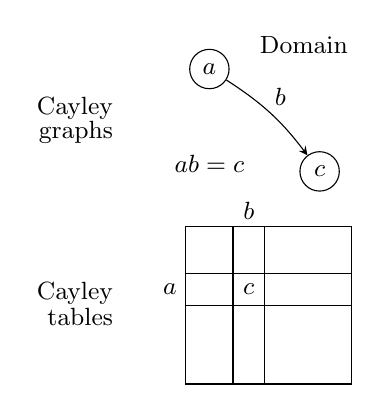
\begin{tikzpicture}
    \tikzstyle{to} = [draw, -stealth]
    \tikzstyle{v} = [circle, draw,inner sep=0pt, minimum size=5mm]
    \tikzstyle{every node}=[font=\small]
    \node[anchor=east] at (-.8,1.15) {Cayley};
    \node[anchor=east] at (-.8,.85) {tables};
    \node[anchor=east] at (-.8,3.5) {Cayley};
    \node[anchor=east] at (-.8,3.2) {graphs};
    \node at (.3,2.8) {\Alert{$ab=c$}};
    \node at (1.5,4.3) {Domain};
    \node (a) at (.3,4) [v] {$a$};
    \node (b) at (1.7,2.7) [v] {$c$};
    \draw[to,bend left=10] (a) to (b); 
    \node at (1.2,3.65) {$b$};
    \draw[thin] (0,0) rectangle (2.1,2);
    \draw[thin] (0,1) -- (2.1,1);
    \draw[thin] (0,1.4) -- (2.1,1.4);
    \draw[thin] (.6,0) -- (.6,2);
    \draw[thin] (1,0) -- (1,2);
    \node at (-.2,1.2) {$a$}; 
    \node at (.8,2.2) {$b$}; 
    \node at (.8,1.2) {$c$};
  \end{tikzpicture}
  %%
  \hspace{3mm}
  %%
  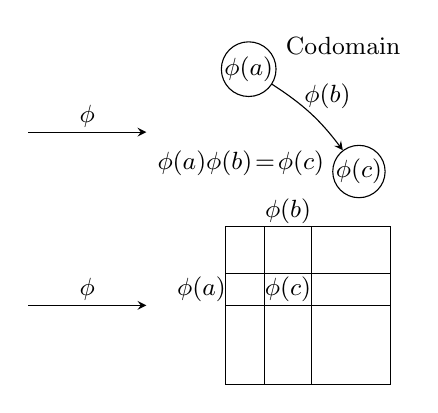
\begin{tikzpicture}
    \tikzstyle{to} = [draw, -stealth]
    \tikzstyle{v} = [circle, draw,inner sep=0pt, minimum size=5mm]
    \tikzstyle{every node}=[font=\small]
    \node at (1.5,4.3) {Codomain};
    \node (a) at (.3,4) [v] {$\phi(a)$};
    \node (b) at (1.7,2.7) [v] {$\phi(c)$};
    \draw[to,bend left=10] (a) to (b);
    \node at (1.3,3.65) {$\phi(b)$};
    \draw[thin,-stealth] (-2.5,3.2) -- (-1,3.2);
    \node at (-1.75,3.4) {$\phi$};
    \draw[thin,-stealth] (-2.5,1) -- (-1,1);
    \node at (-1.75,1.2) {$\phi$};
    \node at (.2,2.8) {\Alert{$\phi(a)\phi(b)\!=\!\phi(c)$}};
    \draw[thin] (0,0) rectangle (2.1,2);
    \draw[thin] (0,1) -- (2.1,1);
    \draw[thin] (0,1.4) -- (2.1,1.4);
    \draw[thin] (.5,0) -- (.5,2);
    \draw[thin] (1.1,0) -- (1.1,2);
    \node at (-.3,1.2) {$\phi(a)$}; 
    \node at (.8,2.2) {$\phi(b)$}; 
    \node at (.8,1.2) {$\phi(c)$};
  \end{tikzpicture}
  \]
  Note that in the Cayley graphs, $b$ and $\phi(b)$ are \Balert{paths}; they
  need not just be edges.
  
\end{frame}
 
%%====================================================================

\begin{frame}{An example} %\Pause

  Consider the function $\phi$ that reduces an integer modulo $5$:
  \[
  \phi\colon\Z\longto\Z_5\,,\qquad \phi(n)=n\pmod{5}.
  \]
  \Pause Since the group operation is \Balert{additive}, the
  ``homomorphism property'' becomes
  \[
  \phi(a+b)=\phi(a)+\phi(b)\,.
  \]
  \Pause In plain English, this just says that one can ``first add and then
  reduce modulo $5$,'' OR ``first reduce modulo $5$ and then add.''

  \Pause\vspace{-3mm}

  %%
  %% Homomorphism property: Cayley graphs and Cayley tables, in Z_5
  %%
  \[
  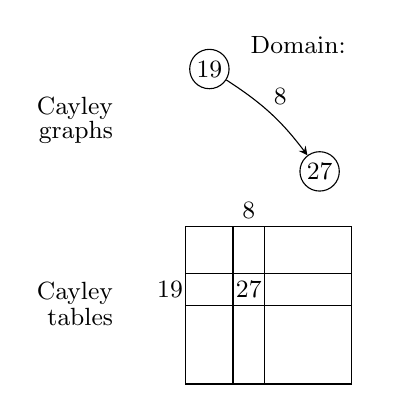
\begin{tikzpicture}
    %%
  \tikzstyle{to} = [draw, -stealth]
  \tikzstyle{v} = [circle, draw,inner sep=0pt, minimum size=5mm]
  \tikzstyle{every node}=[font=\small]
  %%
    \node[anchor=east] at (-.8,1.15) {Cayley};
    \node[anchor=east] at (-.8,.85) {tables};
    \node[anchor=east] at (-.8,3.5) {Cayley};
    \node[anchor=east] at (-.8,3.2) {graphs};
    \node at (1.5,4.3) {Domain: $\Z$};
    \node (a) at (.3,4) [v] {$19$};
    \node (b) at (1.7,2.7) [v] {$27$};
    \draw[to,bend left=10] (a) to (b); 
    \node at (1.2,3.65) {$8$};
    \draw[thin] (0,0) rectangle (2.1,2);
    \draw[thin] (0,1) -- (2.1,1);
    \draw[thin] (0,1.4) -- (2.1,1.4);
    \draw[thin] (.6,0) -- (.6,2);
    \draw[thin] (1,0) -- (1,2);
    \node at (-.2,1.2) {$19$}; 
    \node at (.8,2.2) {$8$}; 
    \node at (.8,1.2) {$27$};
  \end{tikzpicture}
  %%
  \hspace{3mm}
  %%
  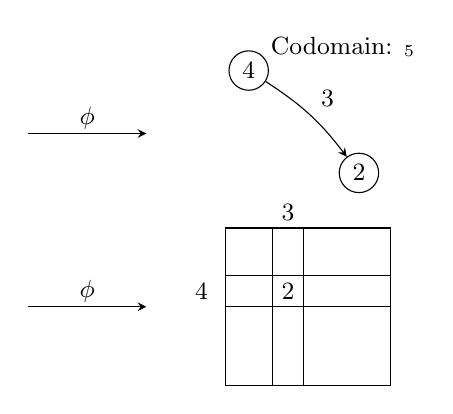
\begin{tikzpicture}
    \tikzstyle{to} = [draw, -stealth]
  \tikzstyle{v} = [circle, draw,inner sep=0pt, minimum size=5mm]
  \tikzstyle{every node}=[font=\small]
    \node at (1.5,4.3) {Codomain: $\Z_5$};
    \node (a) at (.3,4) [v] {$4$};
    \node (b) at (1.7,2.7) [v] {$2$};
    \draw[to,bend left=10] (a) to (b);
    \node at (1.3,3.65) {$3$};
    \draw[thin,-stealth] (-2.5,3.2) -- (-1,3.2);
    \node at (-1.75,3.4) {$\phi$};
    \draw[thin,-stealth] (-2.5,1) -- (-1,1);
    \node at (-1.75,1.2) {$\phi$};
    \draw[thin] (0,0) rectangle (2.1,2);
    \draw[thin] (0,1) -- (2.1,1);
    \draw[thin] (0,1.4) -- (2.1,1.4);
    \draw[thin] (.6,0) -- (.6,2);
    \draw[thin] (1,0) -- (1,2);
    \node at (-.3,1.2) {$4$}; 
    \node at (.8,2.2) {$3$}; 
    \node at (.8,1.2) {$2$};
  \end{tikzpicture}
  \]
  
\end{frame}

%%====================================================================
\section{Types of homomorphisms!}
%%====================================================================

\begin{frame}{Injective homomorphisms aka embeddings} 
  
  Consider the following homomorphism $\theta\colon\Z_3\to C_6$,
  defined by $\theta(n)=r^{2n}$:
  %%
  %% Embedding of Cayley diagrams and lattices: C_3-->C_6.
  %%
  \[
  %%
  \begin{tikzpicture}[scale=.6]
  \tikzstyle{v} = [circle, draw, fill=lightgray,inner sep=0pt, minimum size=3.5mm]
  \tikzstyle{v-y} = [circle, draw, fill=vYellow,inner sep=0pt, minimum size=3.5mm]
  \tikzstyle{vFaded} = [circle, draw, gray,fill=lightgray,inner sep=0pt, minimum size=3.5mm]
%\tikzstyle{v-g} = [circle, draw, fill=green!75!black,inner sep=0pt, 
%  minimum size=6mm]
  \tikzstyle{to} = [draw, dashed, ultra thick, -stealth]
  \tikzstyle{r3} = [draw, very thick, eRed, -stealth,bend right=38]
  \tikzstyle{r6} = [draw, very thick, eRed, -stealth,bend right=14]
  %%
   \begin{scope}[shift={(0,1)}]
     \tikzstyle{every node}=[font=\small]
    \node (0) at (0:1) [v] {$0$};
    \node (1) at (120:1) [v] {$1$};
    \node (2) at (240:1) [v] {$2$};
    \draw [r3] (0) to (1);
    \draw [r3] (1) to (2);
    \draw [r3] (2) to (0);
    \end{scope}
    %%
    \begin{scope}[shift={(5,0)}]
      \tikzstyle{every node}=[font=\small]
      \node (e) at (0:1.5) [v-y] {$1$};
      \node (r) at (60:1.5) [v] {$r$};
      \node (r2) at (120:1.5) [v-y] {$r^2$};
      \node (r3) at (180:1.5) [v] {$r^3$};
      \node (r4) at (240:1.5) [v-y] {$r^4$};
      \node (r5) at (300:1.5) [v] {$r^5$};
      \path[r6] (e) to (r);
      \path[r6] (r) to (r2);
      \path[r6] (r2) to (r3);
      \path[r6] (r3) to (r4);
      \path[r6] (r4) to (r5);
      \path[r6] (r5) to (e);
    \end{scope}
    \draw[to] (0) to (e);
    \draw[to] (1) to (r2);
    \draw[to] (2) to (r4);
    %%
    \begin{scope}[shift={(10,-2)},,shorten >= -2pt, shorten <= -2pt,scale=1.4]    \tikzstyle{every node}=[font=\normalsize]
      \node (0) at (0,0) {$\<0\>$};
      \node (Z3) at (0,1.75) {$\Z_3$};
      \draw (0) to (Z3);
      \draw[right hook-stealth,ultra thick,dashed] (.5,.866) to (2,.866);
    \end{scope}
    \begin{scope}[shift={(14.25,-2)},shorten >= -2pt, shorten <= -2pt,scale=1.4]
    \tikzstyle{every node}=[font=\normalsize]
      \node[faded] (C6) at (0,3) {$C_6$};
      \node(r2) at (-.75,1.75) {$\<r^2\>$};
      \node[faded] (r3) at (.75,1.25) {$\<r^3\>$};
      \node(1) at (0,0) {$\<1\>$};
      \draw[faded] (C6)--(r2); 
      \draw[faded] (C6)--(r3); 
      \draw (r2)--(1); 
      \draw[faded] (r3)--(1); 
    \end{scope}
  \end{tikzpicture}
  \]
  
  \Pause
  
  Note that $\theta(a+b)=\theta(a)\theta(b)$. The
  red arrow in $\Z_3$ gets mapped to the 2-step path in $C_6$. 
  
  \medskip\Pause
  
  A homomorphism $\phi\colon G\to H$ that is \Alert{one-to-one} or \Alert{injective} is an \Alert{embedding}: the group $G$ ``embeds'' into $H$ as a subgroup. \Galert{Optional: write $\phi\colon G\into H$}.

  \begin{block}{Formally:}
    A homomorphism $\phi\colon G\to H$ is \Alert{1-1} or \Alert{injective} if ``every output comes from only one input'':

    \[\text{if } \phi(g_1) = \phi(g_2)\text{, then }g_1 = g_2.\]\pause
    ``If two outputs are the same, then actually the two inputs were the same.''
  \end{block}
  
\end{frame}

%%====================================================================

\begin{frame}{Surjective homomorphisms}
  Consider the homomorphism $\alpha: Q_8 \to V_4 = \<a, b\rangle$, defined by $\alpha(i) = a$ and $\alpha(j) = b$.

  \medskip \pause

  Where does $\alpha$ send everything else in $Q_8$? \pause
  
  \[
    \begin{tikzpicture}[scale=1]
      %%
      \tikzstyle{every node}=[font=\small]
      \tikzstyle{to} = [draw, dashed, ultra thick, -stealth]
      %%
      \begin{scope}[shift={(0,0)}]
        \draw[cosetBlue, fill=cosetBlue] (45:1) circle (.35);
        \draw[cosetBlue, fill=cosetBlue] (135:1) circle (.35);
        \draw[cosetBlue, fill=cosetBlue] (-45:1) circle (.35);
        \draw[cosetBlue, fill=cosetBlue] (-135:1) circle (.35);
        \draw[cosetBlue, fill=cosetBlue] (45:2) circle (.35);
        \draw[cosetBlue, fill=cosetBlue] (135:2) circle (.35);
        \draw[cosetBlue, fill=cosetBlue] (-45:2) circle (.35);
        \draw[cosetBlue, fill=cosetBlue] (-135:2) circle (.35);
        \draw[cosetBlue, fill=cosetBlue,rotate=45] (1,.35) rectangle (2,-.35);
        \draw[cosetBlue, fill=cosetBlue,rotate=135] (1,.35) rectangle (2,-.35);
        \draw[cosetBlue, fill=cosetBlue,rotate=-45] (1,.35) rectangle (2,-.35);
        \draw[cosetBlue, fill=cosetBlue,rotate=-135] (1,.35) rectangle (2,-.35);
        \node (1) at (135:2) [v] {$1$};
        \node (i) at (45:2) [v] {$i$};
        \node (k) at (-45:2) [v] {$k$};
        \node (j) at (-135:2) [v] {$j$};
        \node (-1) at (135:1) [v] {$-1$};
        \node (-i) at (45:1) [v] {$-i$};
        \node (-k) at (-45:1) [v] {$-k$};
        \node (-j) at (-135:1) [v] {$-j$};
        %%
        \path[b] (1) to (i);
        \path[b] (i) to (-1);
        \path[b] (-1) to (-i);
        \path[b] (-i) to (1);
        %%
        \path[b] (-j) to (-k);
        \path[b] (-k) to (j);
        \path[b] (j) to (k);
        \path[b] (k) to (-j);
        %%
        \path[r] (-k) to (-i);
        \path[r] (-i) to (k);
        \path[r] (k) to (i);
        \path[r] (i) to (-k);
        %% 
        \path[r] (1) to (j);
        \path[r] (j) to (-1);
        \path[r] (-1) to (-j);
        \path[r] (-j) to (1);
        %%
        \draw[gg] (1) to coordinate[pos=0.5] (pm1) (-1);
        \draw[gg] (i) to coordinate[pos=0.5] (pmi) (-i);
        \draw[gg] (j) to coordinate[pos=0.5] (pmj) (-j);
        \draw[gg] (k) to coordinate[pos=0.5] (pmk) (-k);
        %%
        \node at (0,0) {\normalsize $Q_8$};
      \end{scope}
      %%
      \begin{scope}[shift={(4,0)}]
        \node (e) at (135:1) [v] {$e$};
        \node (a) at (45:1) [v] {$a$};
        \node (b) at (-135:1) [v] {$b$};
        \node (ab) at (-45:1) [v] {$ab$};
        \node at (0,0) {$V_4$};
        \path[bb] (e) to (a);
        \path[bb] (b) to (ab);
        \path[rr] (e) to (b);
        \path[rr] (a) to (ab);
      \end{scope}
      \path[to] (pm1) to (e);
      \path[to] (pmi) to (a);
      \path[to] (pmj) to (b);
      \path[to] (pmk) to (ab);
    \end{tikzpicture}
  \] \pause

  If $\phi(G)=H$ (``the image of $\phi$ is the entire codomain''), then $\phi$ is \Balert{onto}, or \Balert{surjective}. 
  
  We call $\phi$ a \Balert{quotient map} (yes, it's related!). \Galert{Optional: write $\phi\colon G\onto H$}. \Pause

  \begin{block}{Formal definition}
    The homomorphism $\phi:G\to H$ is \Balert{onto}, or \Balert{surjective}, if for all $h\in H$, there is some $g \in G$ such that $\phi(g) = h$. 
  \end{block}
  
  
\end{frame}

%%====================================================================

\begin{frame}{An example that is neither an embedding nor a quotient} \smallskip

  Consider the homomorphism $\phi\colon Q_8\to A_4$ defined by
  \[
  \phi(i)=(12)(34),\qquad \phi(j)=(13)(24).
  \]
  Using the property of homomorphisms, compute $\phi$ of every other element of $Q_8$. \pause
  %%
  %% Homomorphism Q_8-->A_4 (Cayley diagrams)
  %%
  \[
  \begin{tikzpicture}[scale=1]
    \begin{scope}[shift={(0,0)}]
      \tikzstyle{every node}=[font=\small]
      \node (1) at (135:2) [v] {$1$};
      \node (i) at (45:2) [v] {$i$};
      \node (k) at (-45:2) [v] {$k$};
      \node (j) at (-135:2) [v] {$j$};
      \node (-1) at (135:1) [v] {$-1$};
      \node (-i) at (45:1) [v] {$-i$};
      \node (-k) at (-45:1) [v] {$-k$};
      \node (-j) at (-135:1) [v] {$-j$};
      %%
      \path[b] (1) to (i);
      \path[b] (i) to (-1);
      \path[b] (-1) to (-i);
      \path[b] (-i) to (1);
      %%
      \path[b] (-j) to (-k);
      \path[b] (-k) to (j);
      \path[b] (j) to (k);
      \path[b] (k) to (-j);
      %%
      \path[r] (-k) to (-i);
      \path[r] (-i) to (k);
      \path[r] (k) to (i);
      \path[r] (i) to (-k);
      %% 
      \path[r] (1) to (j);
      \path[r] (j) to (-1);
      \path[r] (-1) to (-j);
      \path[r] (-j) to (1);
      %%
      \path[gg] (1) to (-1);
      \path[gg] (j) to (-j);
      \path[gg] (i) to (-i);
      \path[gg] (k) to (-k);
      %%
      \node at (0,0) {\normalsize $\bm{G=Q_8}$};
      \draw[->] (1.75,0) -- (5.25,0) node[midway,above]{\normalsize $\phi$};
    \end{scope}
    %%
    \begin{scope}[shift={(7.25,0)},scale=.75,bend angle=55]
      \tikzstyle{every node}=[font=\small]
      \tikzstyle{v-light} = [circle, draw, gray, fill=lightgray,inner sep=0pt, 
        minimum size=5.5mm]
      %%
      \begin{scope}[shift={(0:2)}]
        \node at (0,1.75) {\normalsize $\bm{H=A_4}$};
        \node (e) at (-.75,.75) [v] {$e$};
        \node (x) at (.75,.75) [v] {$x$};
        \node (z) at (-.75,-.75) [v] {$z$};
        \node (y) at (.75,-.75) [v] {$y$};
      \end{scope}
      %%
      \begin{scope}[shift={(120:2)}]
        \node[v-light] (a) at (-.75,.75) [v] {$a$};
        \node[v-light] (c) at (.75,.75) [v] {$c$};
        \node[v-light] (d) at (-.75,-.75) [v] {$d$};
        \node[v-light] (b) at (.75,-.75) [v] {$b$};
        \draw [bbFaded] (a) to (c);
        \draw [bbFaded] (d) to (b);
        \draw [rrFaded] (a) to (d);
        \draw [rrFaded] (c) to (b);
      \end{scope}
      %%
      \begin{scope}[shift={(240:2)}]
        \node[v-light] (dd) at (.75,-.75) [v] {$d^2$};
        \node[v-light] (bb) at (.75,.75) [v] {$b^2$};
        \node[v-light] (aa) at (-.75,.75) [v] {$a^2$};
        \node[v-light] (cc) at (-.75,-.75) [v] {$c^2$}; 
        \draw [bbFaded] (aa) to (bb);
        \draw [bbFaded] (cc) to (dd);
        \draw [rrFaded] (aa) to (cc);
        \draw [rrFaded] (bb) to (dd);
      \end{scope}
      %%
      \draw [gFaded] (x) to [bend right=20] (b);
      \draw [gFaded] (e) to [bend right=20] (a);
      \draw [gFaded] (z) to [bend right=7] (c);
      \draw [gFaded] (y) to [bend right=5] (d);
      \draw [gFaded] (a) to [bend right=25] (aa);
      \draw [gFaded] (b) to [bend right=8] (cc);
      \draw [gFaded] (c) to [bend right=22] (dd);
      \draw [gFaded] (d) to [bend right=10] (bb);
      \draw [gFaded] (aa) to [bend right=10] (e);
      \draw [gFaded] (bb) to [bend right=25] (y);
      \draw [gFaded] (cc) to [bend right=25] (x);
      \draw [gFaded] (dd) to [bend right=10] (z);
      \draw [bb] (e) to (x);
      \draw [bb] (z) to (y);
      \draw [rr] (e) to (z);
      \draw [rr] (x) to (y);
      \node at (0:2) {\normalsize $\Image(\phi)$};
    \end{scope}
  \end{tikzpicture}
  \]
  
\end{frame}

%%====================================================================

\begin{frame}{Isomorphisms and automorphisms}

  Note that the words \Alert{injective} and \Balert{surjective} aren't only used in abstract algebra. \pause

  \begin{block}{Definition}
    If a function is both \Alert{injective} and
    \Balert{surjective}, then it is called \Palert{bijective} (or \Palert{a bijection}).
  \end{block} \pause
  \begin{block}{Okay, smartass, what's an isomorphism?} \pause
    Let $G$, $H$ be groups. An \textbf{isomorphism} $\phi: G \to H$ is a \Palert{bijective} \Balert{homomorphism}. \pause

    \smallskip

    $G$ is \textbf{isomorphic} to $H$, written $G\cong H$, if there is an isomorphism between $G$ and $H$.
  \end{block} \pause
  \begin{block}{Definition}
    An \textbf{automorphism} is an isomorphism from a group to itself.
  \end{block}
\end{frame}

%%====================================================================

\begin{frame}{An example of an isomorphism}

  We have already seen that $D_3$ is isomorphic to $S_3$. \medskip\Pause 
  
  This means that there's a bijective correspondence $f\colon D_3\to S_3$. \medskip\Pause
  
  But not just any bijection will do. \Pause Intuitively (but also for order reasons), \smallskip
  \begin{itemize}
  \item $(123)$ and $(132)$ should be the rotations \smallskip\Pause
  \item $(12)$, $(13)$, and $(23)$ should be the reflections \smallskip\Pause
  \item The identity permutation must be the identity symmetry. \smallskip\Pause
  \end{itemize}
  
  It is easy to verify that the following is an isomorphism:
  \[
  \phi\colon D_3\longto S_3,\qquad \phi(r)=(123),\quad\phi(f)=(23).
  \]
  
  \vspace{-5mm}

  %%
  %% 2 Cayley graphs of S_3, and the triangle
  %%

  \[
  \begin{tikzpicture}[scale=.55]
  \colorlet{color1}{actBlue}
  \colorlet{color2}{actGreen}
  \colorlet{color3}{vPurple}
  \tikzstyle{v} = [circle, draw, fill=lightgray,inner sep=0pt, 
    minimum size=3.5mm]
    \begin{scope}[shift={(0,0)},scale=.9]
      \tikzstyle{every node}=[font=\footnotesize]
      \tikzstyle{r-in} = [draw, very thick, eRed,-stealth,bend left=35]
      \tikzstyle{r-out} = [draw, very thick, eRed,-stealth,bend right=48]
      \node (e) at (0:2.4) [v] {$1$};
      \node (r) at (120:2.4) [v] {$r$};
      \node (r2) at (240:2.4) [v] {$r^2$};
      \node (f) at (0:1) [v] {$f$};
      \node (r2f) at (240:1) [v] {$r^2\!f$};
      \node (rf) at (120:1) [v] {$rf$};
      \draw [r-out] (e) to  (r);
      \draw [r-out] (r) to (r2);
      \draw [r-out] (r2) to (e);
      \draw [r-in] (f) to (r2f);
      \draw [r-in] (r2f) to (rf);
      \draw [r-in] (rf) to (f);
      \draw [bb] (e) to (f);
      \draw [bb] (r) to (rf);
      \draw [bb] (r2) to (r2f);
      \node at (0,0) {\normalsize $D_3$};
    \end{scope}
    %%
    \begin{scope}[shift={(6.5,0)}]
      \tikzstyle{v} = [circle, draw, fill=lightgray,inner sep=0pt, 
    minimum size=4.5mm]
      \tikzstyle{every node}=[font=\scriptsize]
      \node (e) at (90:2) [v] {$e$};
      \node (t) at (30:2) [v] {$(23)$};
      \node (ts) at (-30:2) [v] {$(\!123\!)$};
      \node (sts) at (-90:2) [v] {$(13)$};
      \node (st) at (-150:2) [v] {$(\!132\!)$};
      \node (s) at (150:2) [v] {$(12)$};
      \path[bb] (e) to (t);
      \path[gg] (t) to (ts);
      \path[bb] (ts) to (sts);
      \path[gg] (st) to (sts);
      \path[bb] (s) to (st);
      \path[gg] (e) to (s);
      \node at (0,0) {\normalsize $S_3$};
    \end{scope}
    %%
    \begin{scope}[shift={(12,-.75)},scale=1.5]
      \draw[dashed,thick,eBlue] (.5,1.5) to (.5,-.8);
      \draw[dashed,thick,ePurple] (-.5,-.307) to (1.5,.921);
      \draw[dashed,thick,eGreen] (-.5,.921) to (1.5,-.307);
      \draw[color1,fill=color1] (.5,.307)--(.25,.433)--(.5,.866)--(.75,.433)--cycle;
      \draw[color2,fill=color2] (.5,.307)--(.75,.433)--(1,0)--(.5,0)--cycle;
      \draw[color3,fill=color3] (.5,.307)--(.25,.433)--(0,0)--(.5,0)--cycle;
      \draw [black] (0,0)--(.5,.866)--(1,0)--cycle;
      \draw (.5,.55) node {$\mathbf{1}$}; 
      \draw (.3,.2) node {$\mathbf{2}$};\draw (.7,.2) node {$\mathbf{3}$};
      \node[xBlue] at (.5,1.75) {$f\mapsto(23)$};
      \node[xPurple] at (1.7,1.25) {$(13)$};
      \node[xGreen] at (-.8,1.25) {$(12)$};
      \draw[-stealth,eRed] (1.5,-.5) to[very thick,bend right=60] (1.7,.2);
      \node[xRed] at (2.2,-.7) {$r\mapsto(123)$};
    \end{scope}
  \end{tikzpicture}
  \]
  
  \Pause However, there are other isomorphisms between these groups. 
  
\end{frame}


%%====================================================================
\section{Properties of homomorphisms!}
%%====================================================================

\begin{frame}{Some basic properties of homomorphisms}
  \begin{block}{Proposition}
    For any homomorphism $\phi\colon G\to H$: \Pause
    \begin{enumerate}[(i)]
    \item ``{$\phi$ sends the identity to the identity}'' 
    \hfill \pause $\phi(1_G) = 1_H$ \pause
    \item ``{$\phi$ sends inverses to inverses}''
    \hfill \pause $\phi(g\inv) = \phi(g)\inv$ \pause
    \item ``{$\phi$ sends powers to powers}'' \pause
    \item ``{$\phi$ sends orbits to orbits}'' \pause
    \item ``{$\phi$ sends conjugates to conjugates}'' \pause
    \item ``{$\phi$ is determined by what it does to generators}'' \pause
    \end{enumerate}
  \end{block}
  \medskip
  What other properties along these lines can you conjecture? \pause
  \begin{exampleblock}{Homework}
    If $|g|$ is finite, then $|\phi(g)|$ must divide $|g|$.
  \end{exampleblock}
\end{frame}

%%====================================================================

\begin{frame}{A word of caution} %\Pause
  
  Just because a homomorphism $\phi\colon G\to H$ is determined by the
  image of its generators does \emph{not} mean that every such image
  will work.
  
  \medskip\Pause
  
  For example, let's try to define a homomorphism $\phi\colon
  \Z_3\to\Z_4$ by $\phi(1)=1$. \Pause Then we get \vspace{-2mm}
  \[
  \def\arraystretch{1.75}
  \begin{array}{l}
    \phi(2)\Pause=\phi(1+1)\Pause=\phi(1)+\phi(1)\Pause=2,\qquad\Pause
    \\ \phi(0)\Pause=\phi(1+1+1)\Pause=\phi(1)+\phi(1)+\phi(1)\Pause=3\neq
    0. \Pause
  \end{array}
  \]
  This is \emph{impossible}, because $\phi(0)$ must be $0\in\Z_4$.
  
  \medskip\Pause
  
  That's not to say that there isn't a homomorphism
  $\phi\colon\Z_3\to\Z_4$; note that there is always the
  \Alert{trivial homomorphism} between two groups:
  \[
  \phi\colon G\longto H\,,\qquad\phi(g)=1_H\quad\text{for all $g\in G$}.
  \]
  
  \Pause
  
  \begin{exampleblock}{Exercise}
    Show that there is no \Alert{embedding} $\phi\colon\Z_n\into\Z$, for
    $n\geq 2$. That is, \emph{any} such homomorphism must satisfy
    $\phi(1)=0$.
  \end{exampleblock}

\end{frame}


%%====================================================================
\section{Kernels!}
%%====================================================================

\begin{frame}{Kernels}
  \begin{block}{Definition}
    Let $\phi:G\to H$. The \Alert{kernel} of $\phi$ is ``everybody who gets squished down to the identity:'' \pause
    \[\ker(\phi):= \{x\in \phantom{G} \mid \phi(x) = 1\}. \]
  \end{block} \pause
  (I am just going to quickly say the word ``\Alert{nullspace}'' from linear algebra.) \pause
  \begin{exampleblock}{Properties of the kernel}
    \begin{enumerate}[(i)]
      \item $\ker(\phi) \leq G$. \pause
      \item In fact, $\ker(\phi) \normaleq G$! \pause
      \item $\ker(\phi)$ is trivial \Alert{iff} $\phi$ is injective.
    \end{enumerate}
  \end{exampleblock}
\end{frame}

%%====================================================================

\begin{frame}{Example: Find the kernel!} \smallskip

  Consider the homomorphism $\phi\colon Q_8\to A_4$ defined by
  \[
  \phi(i)=(12)(34),\qquad \phi(j)=(13)(24).
  \]
  Who all is in $\ker\phi$?
  %%
  %% Homomorphism Q_8-->A_4 (Cayley diagrams)
  %%
  \[
  \begin{tikzpicture}[scale=1]
    \begin{scope}[shift={(0,0)}]
      \tikzstyle{every node}=[font=\small]
      \node (1) at (135:2) [v] {$1$};
      \node (i) at (45:2) [v] {$i$};
      \node (k) at (-45:2) [v] {$k$};
      \node (j) at (-135:2) [v] {$j$};
      \node (-1) at (135:1) [v] {$-1$};
      \node (-i) at (45:1) [v] {$-i$};
      \node (-k) at (-45:1) [v] {$-k$};
      \node (-j) at (-135:1) [v] {$-j$};
      %%
      \path[b] (1) to (i);
      \path[b] (i) to (-1);
      \path[b] (-1) to (-i);
      \path[b] (-i) to (1);
      %%
      \path[b] (-j) to (-k);
      \path[b] (-k) to (j);
      \path[b] (j) to (k);
      \path[b] (k) to (-j);
      %%
      \path[r] (-k) to (-i);
      \path[r] (-i) to (k);
      \path[r] (k) to (i);
      \path[r] (i) to (-k);
      %% 
      \path[r] (1) to (j);
      \path[r] (j) to (-1);
      \path[r] (-1) to (-j);
      \path[r] (-j) to (1);
      %%
      \path[gg] (1) to (-1);
      \path[gg] (j) to (-j);
      \path[gg] (i) to (-i);
      \path[gg] (k) to (-k);
      %%
      \node at (0,0) {\normalsize $\bm{G=Q_8}$};
      \draw[->] (1.75,0) -- (5.25,0) node[midway,above]{\normalsize $\phi$};
    \end{scope}
    %%
    \begin{scope}[shift={(7.25,0)},scale=.75,bend angle=55]
      \tikzstyle{every node}=[font=\small]
      \tikzstyle{v-light} = [circle, draw, gray, fill=lightgray,inner sep=0pt, 
        minimum size=5.5mm]
      %%
      \begin{scope}[shift={(0:2)}]
        \node at (0,1.75) {\normalsize $\bm{H=A_4}$};
        \node (e) at (-.75,.75) [v] {$e$};
        \node (x) at (.75,.75) [v] {$x$};
        \node (z) at (-.75,-.75) [v] {$z$};
        \node (y) at (.75,-.75) [v] {$y$};
      \end{scope}
      %%
      \begin{scope}[shift={(120:2)}]
        \node[v-light] (a) at (-.75,.75) [v] {$a$};
        \node[v-light] (c) at (.75,.75) [v] {$c$};
        \node[v-light] (d) at (-.75,-.75) [v] {$d$};
        \node[v-light] (b) at (.75,-.75) [v] {$b$};
        \draw [bbFaded] (a) to (c);
        \draw [bbFaded] (d) to (b);
        \draw [rrFaded] (a) to (d);
        \draw [rrFaded] (c) to (b);
      \end{scope}
      %%
      \begin{scope}[shift={(240:2)}]
        \node[v-light] (dd) at (.75,-.75) [v] {$d^2$};
        \node[v-light] (bb) at (.75,.75) [v] {$b^2$};
        \node[v-light] (aa) at (-.75,.75) [v] {$a^2$};
        \node[v-light] (cc) at (-.75,-.75) [v] {$c^2$}; 
        \draw [bbFaded] (aa) to (bb);
        \draw [bbFaded] (cc) to (dd);
        \draw [rrFaded] (aa) to (cc);
        \draw [rrFaded] (bb) to (dd);
      \end{scope}
      %%
      \draw [gFaded] (x) to [bend right=20] (b);
      \draw [gFaded] (e) to [bend right=20] (a);
      \draw [gFaded] (z) to [bend right=7] (c);
      \draw [gFaded] (y) to [bend right=5] (d);
      \draw [gFaded] (a) to [bend right=25] (aa);
      \draw [gFaded] (b) to [bend right=8] (cc);
      \draw [gFaded] (c) to [bend right=22] (dd);
      \draw [gFaded] (d) to [bend right=10] (bb);
      \draw [gFaded] (aa) to [bend right=10] (e);
      \draw [gFaded] (bb) to [bend right=25] (y);
      \draw [gFaded] (cc) to [bend right=25] (x);
      \draw [gFaded] (dd) to [bend right=10] (z);
      \draw [bb] (e) to (x);
      \draw [bb] (z) to (y);
      \draw [rr] (e) to (z);
      \draw [rr] (x) to (y);
      \node at (0:2) {\normalsize $\Image(\phi)$};
    \end{scope}
  \end{tikzpicture}
  \]
  
\end{frame}

%%====================================================================

\begin{frame}{Preimages}
  Here's a slightly more general version of the idea of the kernel:
  \begin{block}{Definition}
    Let $\phi:G\to H$ and choose a fixed element $h\in H$. 
    
    The \Balert{preimage} of $h$ is ``everybody who gets sent to $h$:''\pause
    \[\phi\inv(h) := \{g\in G\mid \phi(g) = h\}.\] \pause
    Alternative names: \Balert{fiber} above $h$, \Balert{pullback} of $h$
  \end{block} \pause
  Let's go back and look at our example again. \pause 
  \begin{alertblock}{A word of caution:}
    $\phi\inv$ is in general not a function! \pause (Unless\ldots)
  \end{alertblock} \pause
  \begin{exampleblock}{Theorem (homework)}
    \begin{enumerate}[(i)]
      \item The kernel of $\phi$ is the fiber above $1$. \pause
      \item For every element $h\in H$, the fiber above $h$ is a coset of $\ker(\phi)$.
    \end{enumerate}
    
  \end{exampleblock}
\end{frame}

%%====================================================================

\begin{frame}{An example of a quotient} \smallskip
  
  Let's write $C_2 = \<-1\> = \{1,-1\}$. Consider the
  following quotient map:
  \[
  \phi\colon D_4\longonto C_2\,,\qquad\text{ defined by }\;
  \Alert{\phi(r)=1}\,\;\text{ and }\;\Galert{\phi(f)=-1}\,.
  \]
  \vspace{-1mm}\Pause (Check: Is this a homomorphism?) \pause Note that:
  \[
  \phi(r^k)\Pause=\phi(r)^k\Pause=1^k\Pause=1,\qquad\qquad\Pause
  \phi(r^kf)\Pause=\phi(r^k)\phi(f)\Pause=\phi(r)^k\phi(f)\Pause=1^k(-1)
  \Pause=-1.
  \]

  \vspace{-4mm}\Pause

  %%
  %% Cayley table of D_4 and a quotient
  %%
  \[
  \begin{tikzpicture}[scale=0.47]
    \tikzstyle{every node}=[font=\footnotesize]
  %%  
  \newcommand*{\n}{9}%
    %%
    \begin{scope}[shift={(0,0)}]
      \path[fill=tRed] (-.1,8) rectangle ++(1,1);
      \path[fill=tOrange] (-.1,7) rectangle ++(1,1);
      \path[fill=tYellow] (-.1,6) rectangle ++(1,1);
      \path[fill=tLime] (-.1,5) rectangle ++(1,1);
      \path[fill=tGreen] (-.1,4) rectangle ++(1,1);
      \path[fill=tBlue] (-.1,3) rectangle ++(1,1);
      \path[fill=tPurple] (-.1,2) rectangle ++(1,1);
      \path[fill=tPink] (-.1,1) rectangle ++(1,1);
      %%
      \path[fill=tRed] (1,9.1) rectangle ++(1,1);
      \path[fill=tOrange] (2,9.1) rectangle ++(1,1);
      \path[fill=tYellow] (3,9.1) rectangle ++(1,1);
      \path[fill=tLime] (4,9.1) rectangle ++(1,1);
      \path[fill=tGreen] (5,9.1) rectangle ++(1,1);
      \path[fill=tBlue] (6,9.1) rectangle ++(1,1);
      \path[fill=tPurple] (7,9.1) rectangle ++(1,1);
      \path[fill=tPink] (8,9.1) rectangle ++(1,1);
      %
      \path[fill=tRed] (1,8) rectangle ++(1,1);
      \path[fill=tRed] (2,5) rectangle ++(1,1);
      \path[fill=tRed] (3,6) rectangle ++(1,1);
      \path[fill=tRed] (4,7) rectangle ++(1,1);
      \path[fill=tRed] (5,4) rectangle ++(1,1);
      \path[fill=tRed] (6,3) rectangle ++(1,1);
      \path[fill=tRed] (7,2) rectangle ++(1,1);
      \path[fill=tRed] (8,1) rectangle ++(1,1);
      %%
      \path[fill=tOrange] (1,7) rectangle ++(1,1);
      \path[fill=tOrange] (2,8) rectangle ++(1,1);
      \path[fill=tOrange] (3,5) rectangle ++(1,1);
      \path[fill=tOrange] (4,6) rectangle ++(1,1);
      \path[fill=tOrange] (5,3) rectangle ++(1,1);
      \path[fill=tOrange] (6,2) rectangle ++(1,1);
      \path[fill=tOrange] (7,1) rectangle ++(1,1);
      \path[fill=tOrange] (8,4) rectangle ++(1,1);
      %%
      \path[fill=tYellow] (1,6) rectangle ++(1,1);
      \path[fill=tYellow] (2,7) rectangle ++(1,1);
      \path[fill=tYellow] (3,8) rectangle ++(1,1);
      \path[fill=tYellow] (4,5) rectangle ++(1,1);
      \path[fill=tYellow] (5,2) rectangle ++(1,1);
      \path[fill=tYellow] (6,1) rectangle ++(1,1);
      \path[fill=tYellow] (7,4) rectangle ++(1,1);
      \path[fill=tYellow] (8,3) rectangle ++(1,1);
      %%
      \path[fill=tLime] (1,5) rectangle ++(1,1);
      \path[fill=tLime] (2,6) rectangle ++(1,1);
      \path[fill=tLime] (3,7) rectangle ++(1,1);
      \path[fill=tLime] (4,8) rectangle ++(1,1);
      \path[fill=tLime] (5,1) rectangle ++(1,1);
      \path[fill=tLime] (6,4) rectangle ++(1,1);
      \path[fill=tLime] (7,3) rectangle ++(1,1);
      \path[fill=tLime] (8,2) rectangle ++(1,1);
      %%
      \path[fill=tGreen] (1,4) rectangle ++(1,1);
      \path[fill=tGreen] (2,3) rectangle ++(1,1);
      \path[fill=tGreen] (3,2) rectangle ++(1,1);
      \path[fill=tGreen] (4,1) rectangle ++(1,1);
      \path[fill=tGreen] (5,8) rectangle ++(1,1);
      \path[fill=tGreen] (6,5) rectangle ++(1,1);
      \path[fill=tGreen] (7,6) rectangle ++(1,1);
      \path[fill=tGreen] (8,7) rectangle ++(1,1);
      %%
      \path[fill=tBlue] (1,3) rectangle ++(1,1);
      \path[fill=tBlue] (2,2) rectangle ++(1,1);
      \path[fill=tBlue] (3,1) rectangle ++(1,1);
      \path[fill=tBlue] (4,4) rectangle ++(1,1);
      \path[fill=tBlue] (5,7) rectangle ++(1,1);
      \path[fill=tBlue] (6,8) rectangle ++(1,1);
      \path[fill=tBlue] (7,5) rectangle ++(1,1);
      \path[fill=tBlue] (8,6) rectangle ++(1,1);
      %%
      \path[fill=tPurple] (1,2) rectangle ++(1,1);
      \path[fill=tPurple] (2,1) rectangle ++(1,1);
      \path[fill=tPurple] (3,4) rectangle ++(1,1);
      \path[fill=tPurple] (4,3) rectangle ++(1,1);
      \path[fill=tPurple] (5,6) rectangle ++(1,1);
      \path[fill=tPurple] (6,7) rectangle ++(1,1);
      \path[fill=tPurple] (7,8) rectangle ++(1,1);
      \path[fill=tPurple] (8,5) rectangle ++(1,1);
      %%
      \path[fill=tPink] (1,1) rectangle ++(1,1);
      \path[fill=tPink] (2,4) rectangle ++(1,1);
      \path[fill=tPink] (3,3) rectangle ++(1,1);
      \path[fill=tPink] (4,2) rectangle ++(1,1);
      \path[fill=tPink] (5,5) rectangle ++(1,1);
      \path[fill=tPink] (6,6) rectangle ++(1,1);
      \path[fill=tPink] (7,7) rectangle ++(1,1);
      \path[fill=tPink] (8,8) rectangle ++(1,1);
      %%
      \foreach \i in {1,...,\n} {
        \draw [very thin] (\i,1) -- (\i,\n); 
        \draw [very thin] (\i,\n+.1) -- (\i,\n+1.1); 
        \draw [very thin] (1,\i) -- (\n,\i); 
        \draw [very thin] (-.1,\i) -- (.9,\i); 
      } 
      \draw [very thin] (1,\n+.1) rectangle (\n,\n+1.1);
      \draw [very thin] (-.1,1) rectangle (.9,\n); 
      \node at (0.4,8.5) {$1$};
      \node at (0.4,7.5) {$r$};
      \node at (0.4,6.5) {$r^2$};
      \node at (0.4,5.5) {$r^3$}; 
      \node at (0.4,4.5) {$f$}; 
      \node at (0.4,3.5) {$rf$};
      \node at (0.4,2.5) {$r^2\!f$};
      \node at (0.4,1.5) {$r^3\!f$};
      %% 
      \node at (1.5,9.6) {$1$};
      \node at (2.5,9.6) {$r$};
      \node at (3.5,9.6) {$r^2$};
      \node at (4.5,9.6) {$r^3$}; 
      \node at (5.5,9.6) {$f$}; 
      \node at (6.5,9.6) {$rf$};
      \node at (7.5,9.6) {$r^2f$};
      \node at (8.5,9.6) {$r^3f$};
      %%
      \node at (1.5,8.5) {$1$};
      \node at (1.5,7.5) {$r$};
      \node at (1.5,6.5) {$r^2$};
      \node at (1.5,5.5) {$r^3$}; 
      \node at (1.5,4.5) {$f$}; 
      \node at (1.5,3.5) {$rf$};
      \node at (1.5,2.5) {$r^2\!f$};
      \node at (1.5,1.5) {$r^3\!f$};
      %%
      \node at (2.5,8.5) {$r$};
      \node at (2.5,7.5) {$r^2$};
      \node at (2.5,6.5) {$r^3$};
      \node at (2.5,5.5) {$1$}; 
      \node at (2.5,4.5) {$r^3f$}; 
      \node at (2.5,3.5) {$f$};
      \node at (2.5,2.5) {$rf$};
      \node at (2.5,1.5) {$r^2f$};
      %%
      \node at (3.5,8.5) {$r^2$};
      \node at (3.5,7.5) {$r^3$};
      \node at (3.5,6.5) {$1$};
      \node at (3.5,5.5) {$r$}; 
      \node at (3.5,4.5) {$r^2f$}; 
      \node at (3.5,3.5) {$r^3f$};
      \node at (3.5,2.5) {$f$};
      \node at (3.5,1.5) {$rf$};
      %%
      \node at (4.5,8.5) {$r^3$};
      \node at (4.5,7.5) {$1$};
      \node at (4.5,6.5) {$r$};
      \node at (4.5,5.5) {$r^2$}; 
      \node at (4.5,4.5) {$rf$}; 
      \node at (4.5,3.5) {$r^2f$};
      \node at (4.5,2.5) {$r^3f$};
      \node at (4.5,1.5) {$f$};
      %%
      \node at (5.5,8.5) {$f$};
      \node at (5.5,7.5) {$rf$};
      \node at (5.5,6.5) {$r^2f$};
      \node at (5.5,5.5) {$r^3f$}; 
      \node at (5.5,4.5) {$1$}; 
      \node at (5.5,3.5) {$r$};
      \node at (5.5,2.5) {$r^2$};
      \node at (5.5,1.5) {$r^3$};
      %%
      \node at (6.5,8.5) {$rf$};
      \node at (6.5,7.5) {$r^2f$};
      \node at (6.5,6.5) {$r^3f$};
      \node at (6.5,5.5) {$f$}; 
      \node at (6.5,4.5) {$r^3$}; 
      \node at (6.5,3.5) {$1$};
      \node at (6.5,2.5) {$r$};
      \node at (6.5,1.5) {$r^2$};
      %%
      \node at (7.5,8.5) {$r^2f$};
      \node at (7.5,7.5) {$r^3f$};
      \node at (7.5,6.5) {$f$};
      \node at (7.5,5.5) {$rf$}; 
      \node at (7.5,4.5) {$r^2$}; 
      \node at (7.5,3.5) {$r^3$};
      \node at (7.5,2.5) {$1$};
      \node at (7.5,1.5) {$r$};
      %%
      \node at (8.5,8.5) {$r^3f$};
      \node at (8.5,7.5) {$f$};
      \node at (8.5,6.5) {$rf$};
      \node at (8.5,5.5) {$r^2f$}; 
      \node at (8.5,4.5) {$r$}; 
      \node at (8.5,3.5) {$r^2$};
      \node at (8.5,2.5) {$r^3$};
      \node at (8.5,1.5) {$1$};
      %%
    \end{scope}
    %%
    %%
    \begin{scope}[shift={(12,0)}]
      \path[fill=tRed] (-.1,8) rectangle ++(1,1);
      \path[fill=tOrange] (-.1,7) rectangle ++(1,1);
      \path[fill=tYellow] (-.1,6) rectangle ++(1,1);
      \path[fill=tLime] (-.1,5) rectangle ++(1,1);
      \path[fill=tGreen] (-.1,4) rectangle ++(1,1);
      \path[fill=tBlue] (-.1,3) rectangle ++(1,1);
      \path[fill=tPurple] (-.1,2) rectangle ++(1,1);
      \path[fill=tPink] (-.1,1) rectangle ++(1,1);
      %%
      \path[fill=tRed] (1,9.1) rectangle ++(1,1);
      \path[fill=tOrange] (2,9.1) rectangle ++(1,1);
      \path[fill=tYellow] (3,9.1) rectangle ++(1,1);
      \path[fill=tLime] (4,9.1) rectangle ++(1,1);
      \path[fill=tGreen] (5,9.1) rectangle ++(1,1);
      \path[fill=tBlue] (6,9.1) rectangle ++(1,1);
      \path[fill=tPurple] (7,9.1) rectangle ++(1,1);
      \path[fill=tPink] (8,9.1) rectangle ++(1,1);
      %
      \path[fill=tRed] (1,8) rectangle ++(1,1);
      \path[fill=tRed] (2,5) rectangle ++(1,1);
      \path[fill=tRed] (3,6) rectangle ++(1,1);
      \path[fill=tRed] (4,7) rectangle ++(1,1);
      \path[fill=tRed] (5,4) rectangle ++(1,1);
      \path[fill=tRed] (6,3) rectangle ++(1,1);
      \path[fill=tRed] (7,2) rectangle ++(1,1);
      \path[fill=tRed] (8,1) rectangle ++(1,1);
      %%
      \path[fill=tOrange] (1,7) rectangle ++(1,1);
      \path[fill=tOrange] (2,8) rectangle ++(1,1);
      \path[fill=tOrange] (3,5) rectangle ++(1,1);
      \path[fill=tOrange] (4,6) rectangle ++(1,1);
      \path[fill=tOrange] (5,3) rectangle ++(1,1);
      \path[fill=tOrange] (6,2) rectangle ++(1,1);
      \path[fill=tOrange] (7,1) rectangle ++(1,1);
      \path[fill=tOrange] (8,4) rectangle ++(1,1);
      %%
      \path[fill=tYellow] (1,6) rectangle ++(1,1);
      \path[fill=tYellow] (2,7) rectangle ++(1,1);
      \path[fill=tYellow] (3,8) rectangle ++(1,1);
      \path[fill=tYellow] (4,5) rectangle ++(1,1);
      \path[fill=tYellow] (5,2) rectangle ++(1,1);
      \path[fill=tYellow] (6,1) rectangle ++(1,1);
      \path[fill=tYellow] (7,4) rectangle ++(1,1);
      \path[fill=tYellow] (8,3) rectangle ++(1,1);
      %%
      \path[fill=tLime] (1,5) rectangle ++(1,1);
      \path[fill=tLime] (2,6) rectangle ++(1,1);
      \path[fill=tLime] (3,7) rectangle ++(1,1);
      \path[fill=tLime] (4,8) rectangle ++(1,1);
      \path[fill=tLime] (5,1) rectangle ++(1,1);
      \path[fill=tLime] (6,4) rectangle ++(1,1);
      \path[fill=tLime] (7,3) rectangle ++(1,1);
      \path[fill=tLime] (8,2) rectangle ++(1,1);
      %%
      \path[fill=tGreen] (1,4) rectangle ++(1,1);
      \path[fill=tGreen] (2,3) rectangle ++(1,1);
      \path[fill=tGreen] (3,2) rectangle ++(1,1);
      \path[fill=tGreen] (4,1) rectangle ++(1,1);
      \path[fill=tGreen] (5,8) rectangle ++(1,1);
      \path[fill=tGreen] (6,5) rectangle ++(1,1);
      \path[fill=tGreen] (7,6) rectangle ++(1,1);
      \path[fill=tGreen] (8,7) rectangle ++(1,1);
      %%
      \path[fill=tBlue] (1,3) rectangle ++(1,1);
      \path[fill=tBlue] (2,2) rectangle ++(1,1);
      \path[fill=tBlue] (3,1) rectangle ++(1,1);
      \path[fill=tBlue] (4,4) rectangle ++(1,1);
      \path[fill=tBlue] (5,7) rectangle ++(1,1);
      \path[fill=tBlue] (6,8) rectangle ++(1,1);
      \path[fill=tBlue] (7,5) rectangle ++(1,1);
      \path[fill=tBlue] (8,6) rectangle ++(1,1);
      %%
      \path[fill=tPurple] (1,2) rectangle ++(1,1);
      \path[fill=tPurple] (2,1) rectangle ++(1,1);
      \path[fill=tPurple] (3,4) rectangle ++(1,1);
      \path[fill=tPurple] (4,3) rectangle ++(1,1);
      \path[fill=tPurple] (5,6) rectangle ++(1,1);
      \path[fill=tPurple] (6,7) rectangle ++(1,1);
      \path[fill=tPurple] (7,8) rectangle ++(1,1);
      \path[fill=tPurple] (8,5) rectangle ++(1,1);
      %%
      \path[fill=tPink] (1,1) rectangle ++(1,1);
      \path[fill=tPink] (2,4) rectangle ++(1,1);
      \path[fill=tPink] (3,3) rectangle ++(1,1);
      \path[fill=tPink] (4,2) rectangle ++(1,1);
      \path[fill=tPink] (5,5) rectangle ++(1,1);
      \path[fill=tPink] (6,6) rectangle ++(1,1);
      \path[fill=tPink] (7,7) rectangle ++(1,1);
      \path[fill=tPink] (8,8) rectangle ++(1,1);
      %%
      \foreach \i in {1,...,\n} {
        \draw [very thin] (\i,1) -- (\i,\n); 
        \draw [very thin] (\i,\n+.1) -- (\i,\n+1.1); 
        \draw [very thin] (1,\i) -- (\n,\i); 
        \draw [very thin] (-.1,\i) -- (.9,\i); 
      } 
      \draw [very thin] (1,\n+.1) rectangle (\n,\n+1.1);
      \draw [very thin] (-.1,1) rectangle (.9,\n); 
      \node at (0.4,8.5) {$1$};
      \node at (0.4,7.5) {$r$};
      \node at (0.4,6.5) {$r^2$};
      \node at (0.4,5.5) {$r^3$}; 
      \node at (0.4,4.5) {$f$}; 
      \node at (0.4,3.5) {$rf$};
      \node at (0.4,2.5) {$r^2\!f$};
      \node at (0.4,1.5) {$r^3\!f$};
      %% 
      \node at (1.5,9.6) {$1$};
      \node at (2.5,9.6) {$r$};
      \node at (3.5,9.6) {$r^2$};
      \node at (4.5,9.6) {$r^3$}; 
      \node at (5.5,9.6) {$f$}; 
      \node at (6.5,9.6) {$rf$};
      \node at (7.5,9.6) {$r^2f$};
      \node at (8.5,9.6) {$r^3f$};
      %%
      \node at (1.5,8.5) {$1$};
      \node at (1.5,7.5) {$r$};
      \node at (1.5,6.5) {$r^2$};
      \node at (1.5,5.5) {$r^3$}; 
      \node at (1.5,4.5) {$f$}; 
      \node at (1.5,3.5) {$rf$};
      \node at (1.5,2.5) {$r^2\!f$};
      \node at (1.5,1.5) {$r^3\!f$};
      %%
      \node at (2.5,8.5) {$r$};
      \node at (2.5,7.5) {$r^2$};
      \node at (2.5,6.5) {$r^3$};
      \node at (2.5,5.5) {$1$}; 
      \node at (2.5,4.5) {$r^3f$}; 
      \node at (2.5,3.5) {$f$};
      \node at (2.5,2.5) {$rf$};
      \node at (2.5,1.5) {$r^2f$};
      %%
      \node at (3.5,8.5) {$r^2$};
      \node at (3.5,7.5) {$r^3$};
      \node at (3.5,6.5) {$1$};
      \node at (3.5,5.5) {$r$}; 
      \node at (3.5,4.5) {$r^2f$}; 
      \node at (3.5,3.5) {$r^3f$};
      \node at (3.5,2.5) {$f$};
      \node at (3.5,1.5) {$rf$};
      %%
      \node at (4.5,8.5) {$r^3$};
      \node at (4.5,7.5) {$1$};
      \node at (4.5,6.5) {$r$};
      \node at (4.5,5.5) {$r^2$}; 
      \node at (4.5,4.5) {$rf$}; 
      \node at (4.5,3.5) {$r^2f$};
      \node at (4.5,2.5) {$r^3f$};
      \node at (4.5,1.5) {$f$};
      %%
      \node at (5.5,8.5) {$f$};
      \node at (5.5,7.5) {$rf$};
      \node at (5.5,6.5) {$r^2f$};
      \node at (5.5,5.5) {$r^3f$}; 
      \node at (5.5,4.5) {$1$}; 
      \node at (5.5,3.5) {$r$};
      \node at (5.5,2.5) {$r^2$};
      \node at (5.5,1.5) {$r^3$};
      %%
      \node at (6.5,8.5) {$rf$};
      \node at (6.5,7.5) {$r^2f$};
      \node at (6.5,6.5) {$r^3f$};
      \node at (6.5,5.5) {$f$}; 
      \node at (6.5,4.5) {$r^3$}; 
      \node at (6.5,3.5) {$1$};
      \node at (6.5,2.5) {$r$};
      \node at (6.5,1.5) {$r^2$};
      %%
      \node at (7.5,8.5) {$r^2f$};
      \node at (7.5,7.5) {$r^3f$};
      \node at (7.5,6.5) {$f$};
      \node at (7.5,5.5) {$rf$}; 
      \node at (7.5,4.5) {$r^2$}; 
      \node at (7.5,3.5) {$r^3$};
      \node at (7.5,2.5) {$1$};
      \node at (7.5,1.5) {$r$};
      %%
      \node at (8.5,8.5) {$r^3f$};
      \node at (8.5,7.5) {$f$};
      \node at (8.5,6.5) {$rf$};
      \node at (8.5,5.5) {$r^2f$}; 
      \node at (8.5,4.5) {$r$}; 
      \node at (8.5,3.5) {$r^2$};
      \node at (8.5,2.5) {$r^3$};
      \node at (8.5,1.5) {$1$};
      %%
      \filldraw[fill=white,opacity=0.7] 
      (1,1)--(9,1)--(9,9)--(1,9)--cycle;
      \draw[thick] (5,1)--(5,9);
      \draw[thick] (1,5)--(9,5);
      \node at (3,7) {\Large $\mathbf{1}$}; %{\large\bf rotation};
      \node at (7,7) {\Large $\mathbf{-1}$}; %{\large\bf reflection};
      \node at (3,3) {\Large $\mathbf{-1}$}; %{\large\bf reflection};
      \node at (7,3) {\Large $\mathbf{1}$}; %{\large\bf rotation};
    \end{scope}
  \end{tikzpicture}
  \]
  
  \vspace{-4mm}
  
  \[
  \Ker(\phi)=\phi^{-1}(1)=\<r\>\quad (\text{``\emph{rotations}''}),\qquad\qquad
  \phi^{-1}(-1)=f\<r\>\quad (\text{``\emph{reflections}''}).
  \]
  
\end{frame}

%%====================================================================
\section{The end!}
\end{document}
